\documentclass[]{article}
\usepackage{graphicx}
\usepackage[left=1in, right =1in, top =1in ,bottom = 1in]{geometry}
%opening
\title{Sailing robot electronic system tutorial}
\author{Yu Cao}

\begin{document}

\maketitle

\section{Sensors}
\subsection{Inertia Measurement Unit}
Inertia Measurement Unit (usually called IMU) is a passive electro-mechanical sensor that measures linear and angular motion with gyroscope and accelerometer. Integrated with magnetometer and barometer, IMU can provide orientation information for the boat. \\

\textbf{Task.1} Find the data-sheet of Polulu AltIMU-10 v3 and try to answer the following:
 \begin{itemize}
 	\item What is the interface of this sensor?
 	\item What is the operating voltage range of this sensor?
 	\item Draw the orientation of this chip in $xyz$ coordinate.
 \end{itemize}
 
 
\begin{figure}[tbph]
\centering
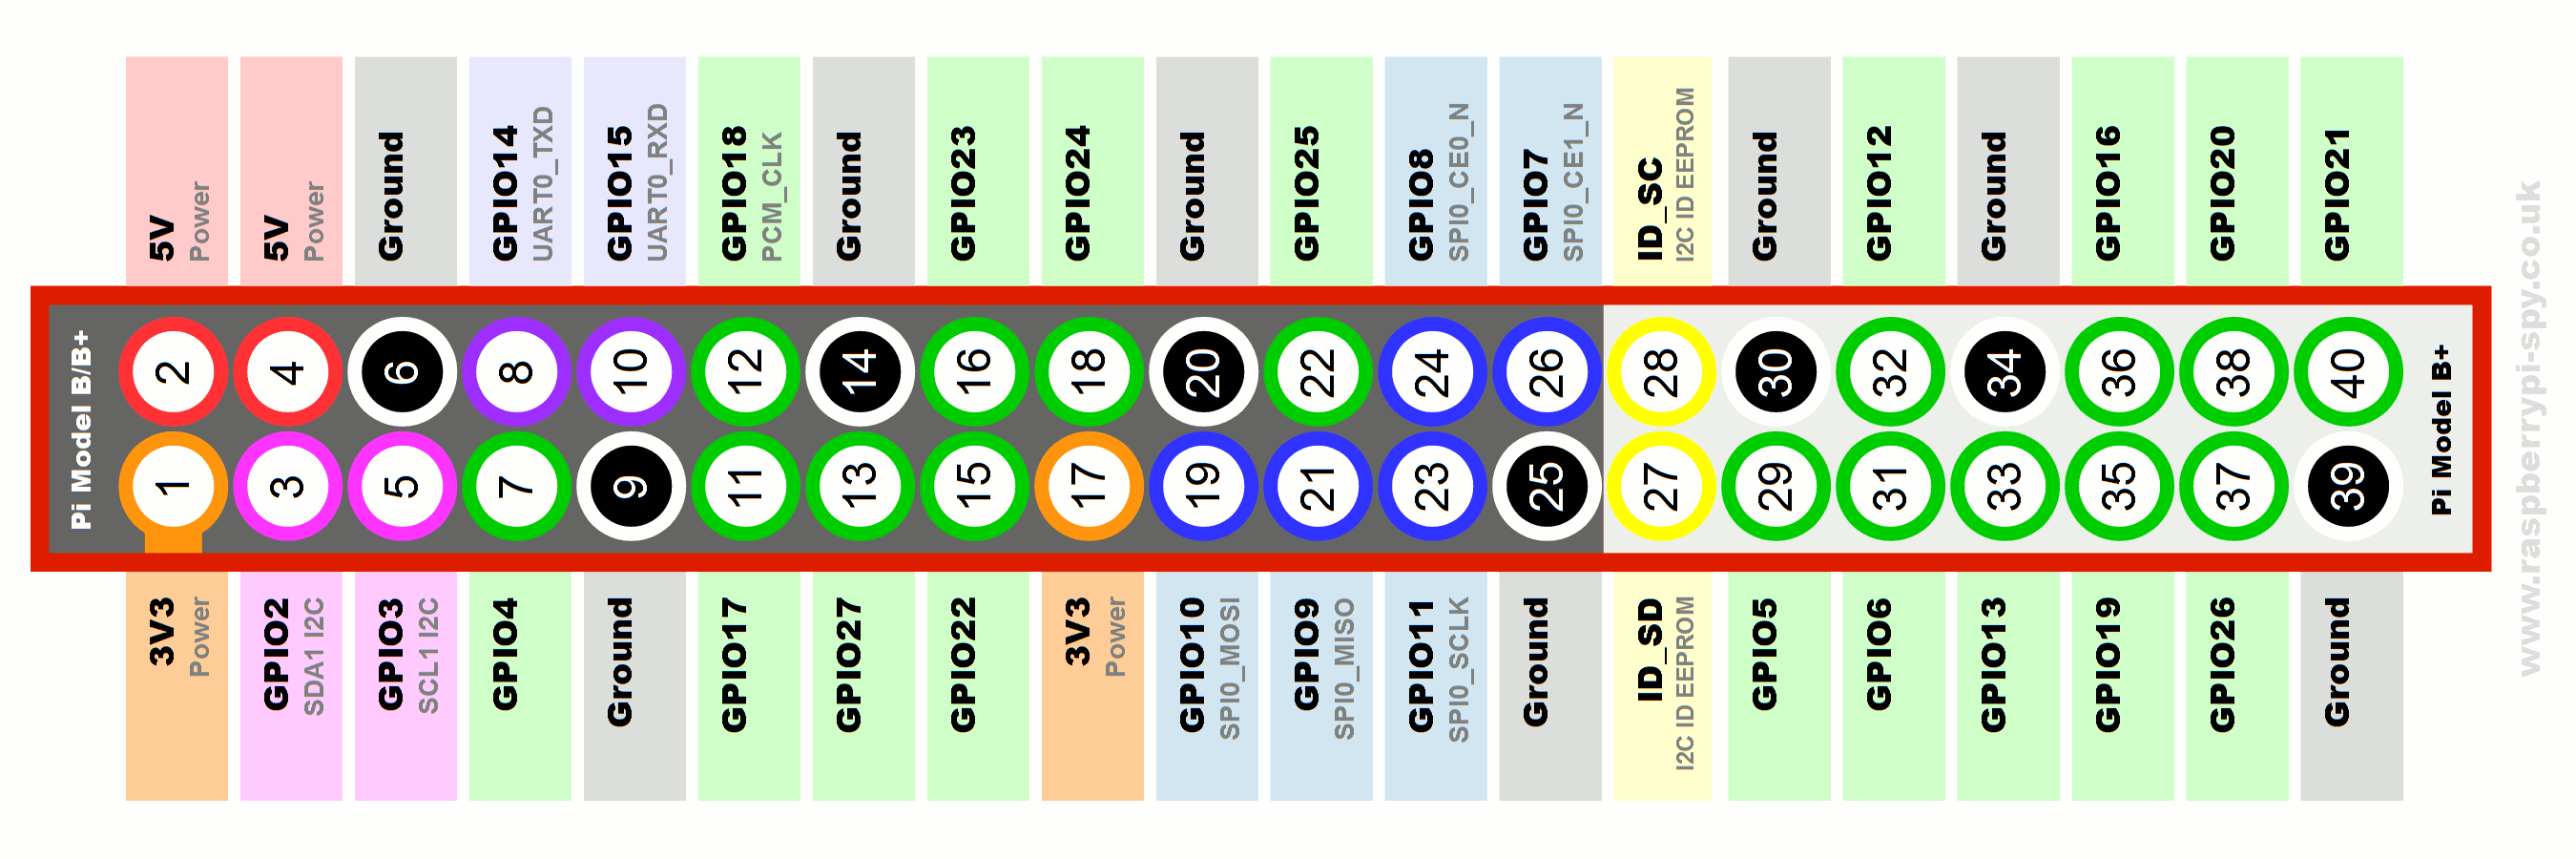
\includegraphics[width=0.7\linewidth]{Raspberry-Pi-GPIO-Layout.png}
\caption{GPIO layout of Raspberry Pi Model B}
\label{fig:raspberry-pi-gpio-layout}
\end{figure}
 
\begin{figure}[tbph]
\centering
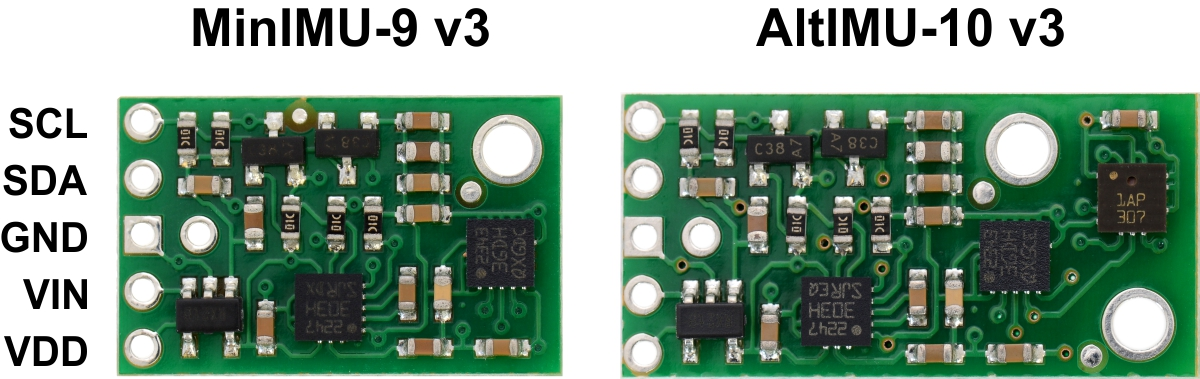
\includegraphics[width=0.5\linewidth]{IMU.jpg}
\caption{Pin layout of AltIMU-10 v3}
\label{fig:0j5187}
\end{figure}

 \textbf{Task.2} Use the given Raspberry PI GPIO and AltIMU-10 v3 layout 
 \begin{itemize}
 	\item Draw the connection line between Raspberry and IMU
 	\item Explain what is SCL, SDA, GND, VIN and VDD
 	\item Search GitHub wiki page to verify your answer
 \end{itemize}


\textbf{Task.3} Design considerations for IMU on boat
\begin{itemize}
	\item Can we use gyroscope reading directly for heading?
	\item Where in the boat is the best place for IMU? Explain with reasons.  
	\item  Can we compensate the IMU reading errors? If so, how to do that? 
\end{itemize}


\subsection{Global Positioning System (GPS)}
Global Positioning System is a satellite based navigation system which can provides location information to users. It now have been widely used in many applications including our autonomous boat. \\

\textbf{Task.1}  Find data sheet of Uputronics u-blox MAX-M8Q and try to answer:
\begin{itemize}
	\item What is the interface of this sensor?
	\item What is the operating voltage range of this sensor?
	\item What is the horizontal position accuracy of this sensor?
\end{itemize}
\begin{figure}[h]
	\centering
	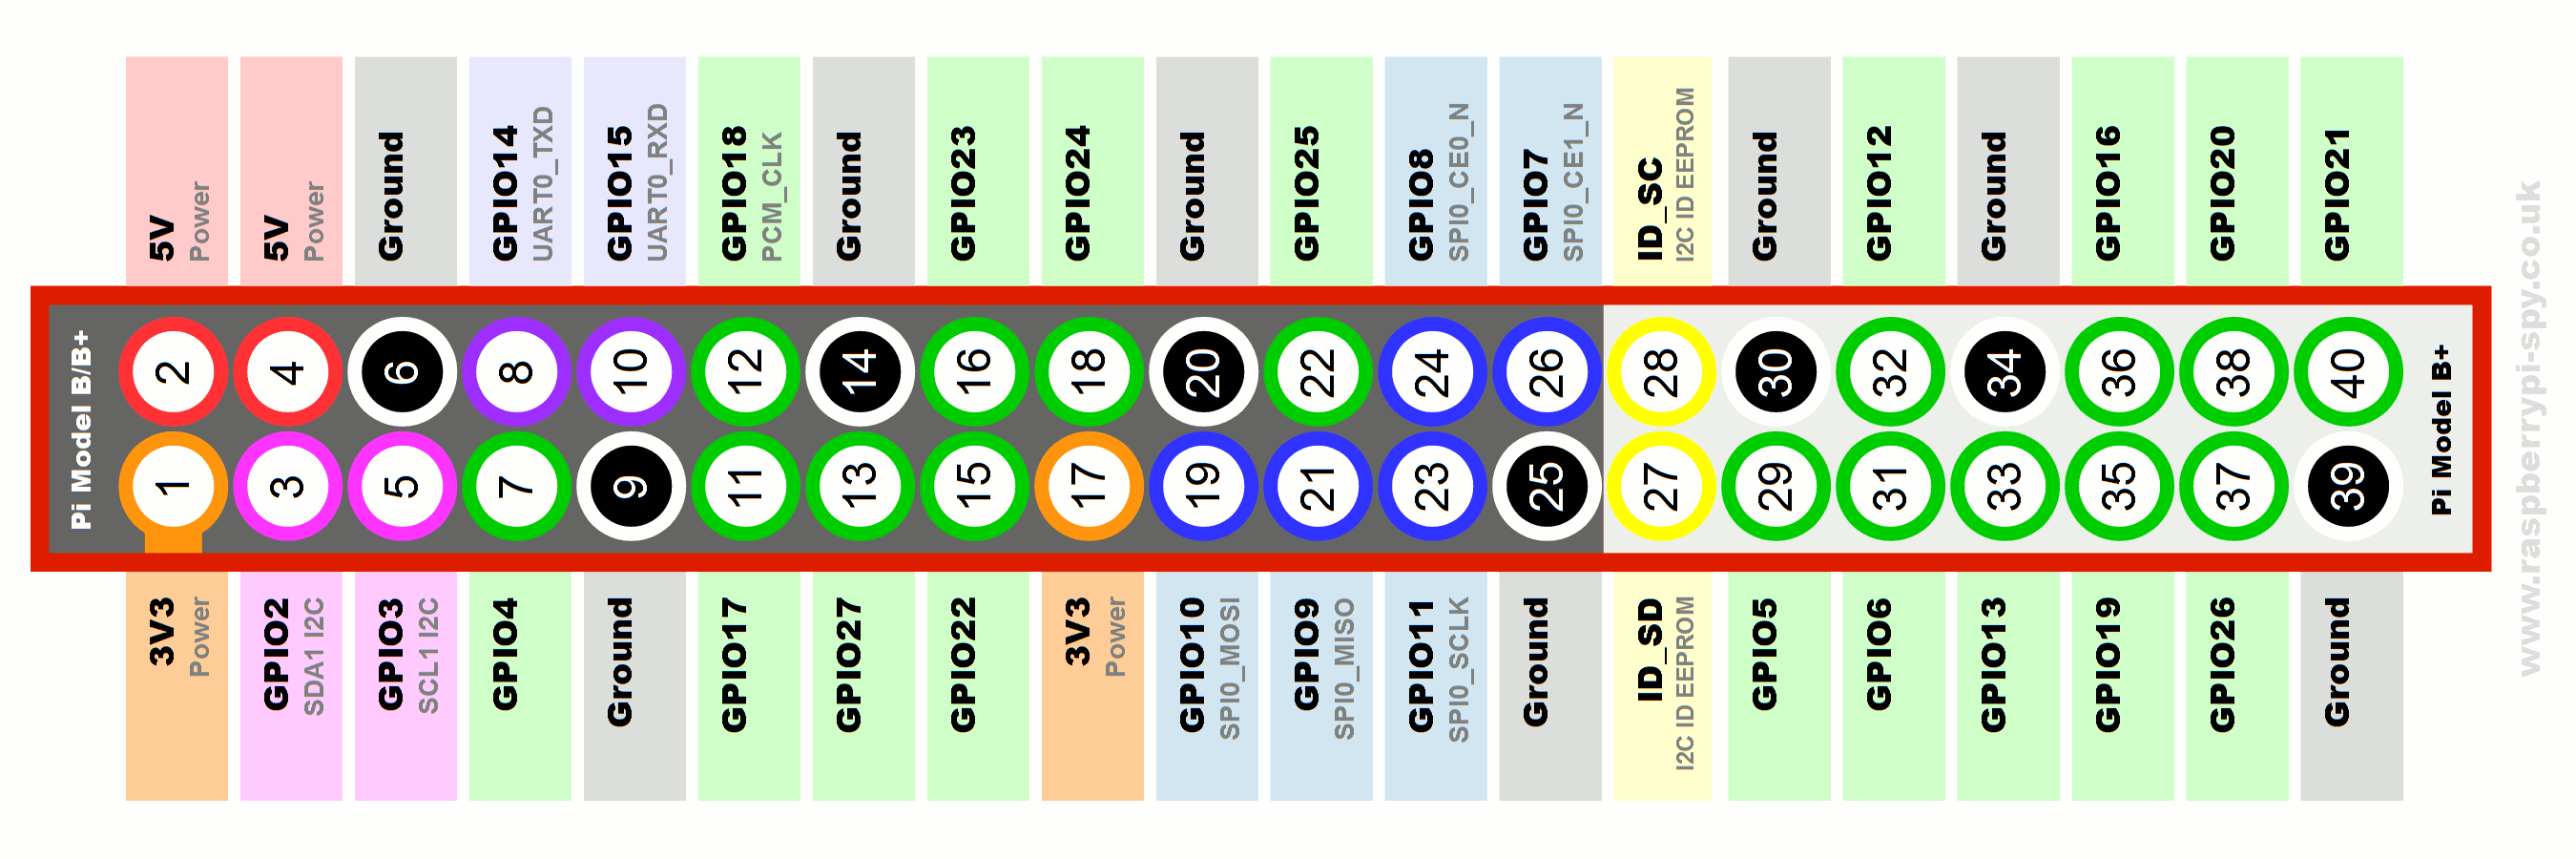
\includegraphics[width=0.7\linewidth]{Raspberry-Pi-GPIO-Layout.png}
	\caption{GPIO layout of Raspberry Pi Model B}
	\label{fig:raspberry-pi-gpio-layout}
\end{figure}
\begin{figure}[h]
\centering
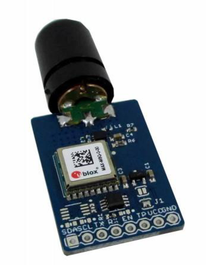
\includegraphics[width=0.3\linewidth]{GPS}
\caption{GPS chip}
\label{fig:gps}
\end{figure}
 \textbf{Task.2} Use the given Raspberry PI GPIO and GPS layout 
 \begin{itemize}
 	\item Draw the connection line between Raspberry and GPS
 	\item Explain what is TX, RX,  GND, EN and TP
 	\item Search GitHub wiki page to verify your answer
 \end{itemize}

\textbf{Task.3} Design considerations for GPS
\begin{itemize}
	\item Where in the boat is the best place for GPS? Explain with reasons.  
	\item  In what kind of price range, we have the best design trade-off between price/performance? 
\end{itemize}

\subsection{Wind direction sensor}
Wind sensor use magnetometer and two pieces of magnets to detect the wind direction. We use built in magnetometer of AltIMU10-v3 so that we have interchangeable sensors to reduce the workload and improve the system redundancy.


\textbf{Task 1.} Quickly review the answer in IMU part:
  \begin{itemize}
  	\item What is the interface of this sensor?
  	\item What is the operating voltage range of this sensor?
  	\item Draw the orientation of this chip in $xyz$ coordinate.
  \end{itemize}
  
  
\begin{figure}[tbph]
\centering
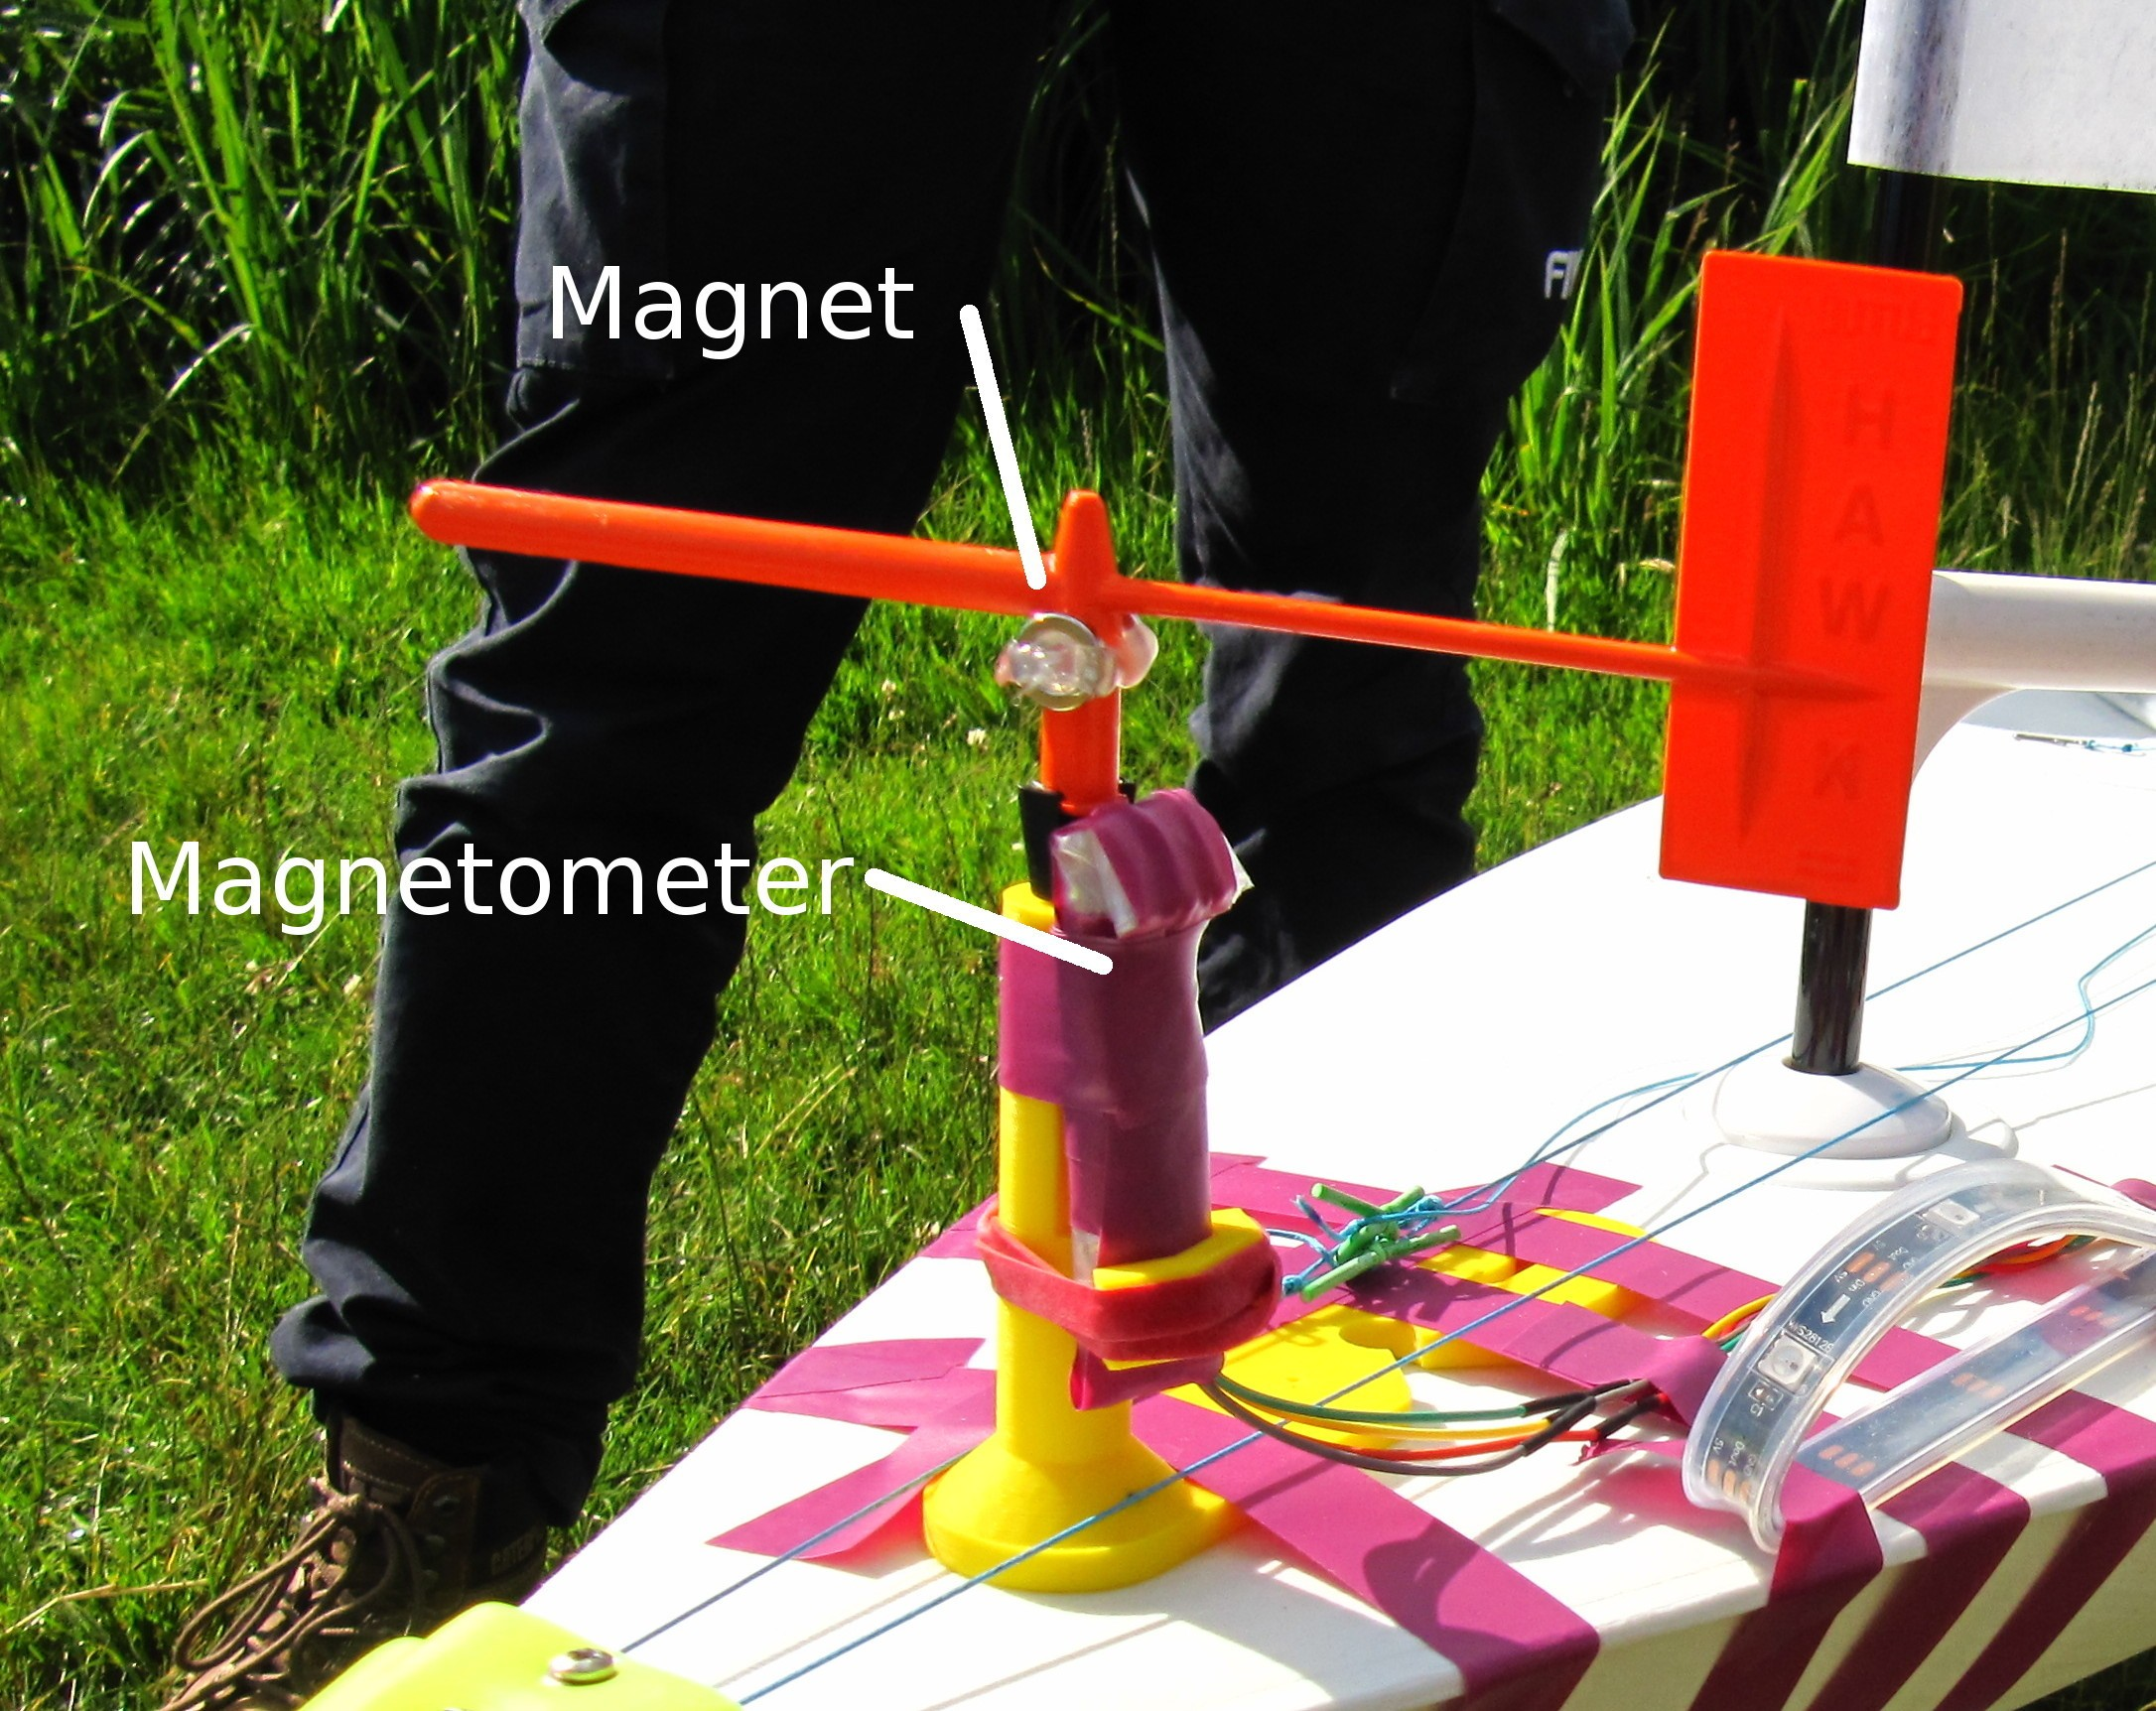
\includegraphics[width=0.7\linewidth]{windsensor}
\caption{"Hand made" wind direction sensor}
\label{fig:windsensor}
\end{figure}
  
 \textbf{Task 2.} Design consideration
 \begin{itemize}
 	\item What is requirement of the wind vane?
 	\item How can you improve our current design?
 \end{itemize}
  

\subsection{Wind speed sensor}

Wind speed sensor is not used on boat. We have an analog maplin wind speed sensor used in conjunction with Arduino UNO. \\

 \textbf{Task 1.} Find data sheet of this sensor
 \begin{itemize}
 	\item Rotate the sensor and listen carefully the switch in side.
 	\item What do you think how this sensor works?
 	\item What is the relationship between pulse and wind speed?
 \end{itemize}

\textbf{Task 2.} How to improve the performance of this sensor?
\begin{itemize}
	\item How ultra-sonic wind speed sensor work?
	\item Does it realistic to use ultrasonic sensor on sailing robot?
	\item What is the best design trade-off ? 
\end{itemize}

\section{Actuators}
\subsection{Sail winch servo}
\begin{figure}[h]
\centering
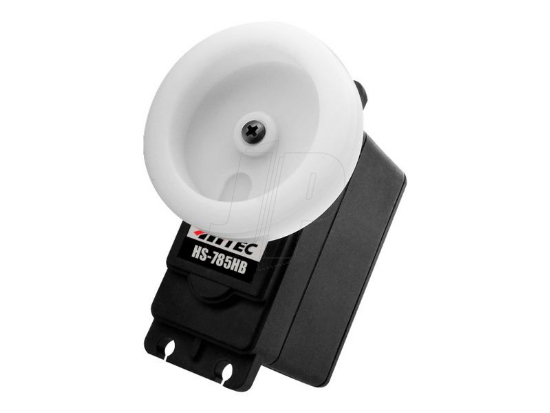
\includegraphics[width=0.7\linewidth]{winch}
\caption{Who am I?}
\label{fig:winch}
\end{figure}
\textbf{Task 1.} Servo control 
\begin{itemize}
	\item How can we control a servo?
	\item What is range of this servo in turns/ degrees?
	\item What signal we send can make servo move to neutral position? 
\end{itemize}

\textbf{Task 2.} Interface and design consideration
\begin{itemize}
	\item How raspberry interface with servos?
	\item What is hardware and software PWM?
	\item How powerful our winch servo should be?
	\item If we are designing a four metres long boat, how can we scale it up?
\end{itemize}


\subsection{Rudder servo}
\begin{figure}[h]
\centering
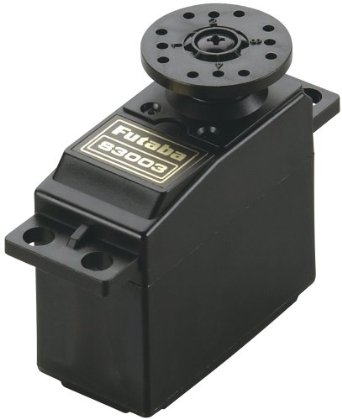
\includegraphics[width=0.4\linewidth]{futaba3003}
\caption{Who am I?}
\label{fig:futaba3003}
\end{figure}
\textbf{Task 1.} Servo control 
\begin{itemize}
	\item How can we control a servo?
	\item What is range of this servo in turns/ degrees?
	\item What signal we send can make servo move to neutral position? 
\end{itemize}

\textbf{Task 2.} Interface and design consideration
\begin{itemize}
	\item How raspberry interface with servos?
	\item What is hardware and software PWM?
	\item How powerful our winch servo should be?
	\item If we are designing a four metres long boat, how can we scale it up?
\end{itemize}

\section{Peripherals}
\subsection{USB camera}

\subsection{WiFi access point}
Try to work out the WiFi password and login Raspberry Pi.
\end{document}
